%	The main skeletal structure
\documentclass[crop,tikz, convert={outext=.svg,command=\unexpanded{/opt/homebrew/bin/pdf2svg \infile\space\outfile}},multi=false]{standalone}%	\documentclass[twocolumn]{report}
% convert={outext=.svg,command=\unexpanded{pdf2svg \infile\space\outfile}} ,multi=false
	\usepackage{setspace}
	\usepackage{graphicx}
		\DeclareGraphicsExtensions{.pdf,.png,.eps,.ps}
	\usepackage{subcaption}
	\usepackage{lscape}
	\usepackage{pifont}
%	\usepackage{bbding}
	\usepackage{multirow}
	\usepackage{longtable}
	\usepackage[version=4]{mhchem}
	\usepackage{xfrac}
	\usepackage{color}
	\usepackage[colorlinks=true]{hyperref}
	\usepackage{gensymb}
	\usepackage{multicol}
		\setlength{\columnseprule}{0.4pt}
		\setlength{\columnsep}{5mm}
\makeatletter 
\newcounter{reaction} 
%%% >> for article << 
%\renewcommand\thereaction{C\,\arabic{reaction}} 
%%% << for article << 
%%% >> for report and book >> 
\renewcommand\thereaction{C\,\thechapter.\arabic{reaction}} 
\@addtoreset{reaction}{chapter} 
%%% << for report and book << 
\newcommand\reactiontag{\refstepcounter{reaction}\tag{\thereaction}} 
\newcommand\reaction@[2][]{\begin{equation}\ce{#2}% 
\ifx\@empty#1\@empty\else\label{#1}\fi% 
\reactiontag\end{equation}} 
\newcommand\reaction@nonumber[1]{\begin{equation*}\ce{#1}% 
\end{equation*}} 
\newcommand\reaction{\@ifstar{\reaction@nonumber}{\reaction@}} 
\makeatother 


	\usepackage[a4paper]{geometry}
	\usepackage{fullpage}
	\usepackage{fancyhdr}
%		\pagestyle{fancy}
%		\lhead{}
%		\chead{}
%		\rhead{\slshape \rightmark}
%		\fancyhead[LO,RE]{\slshape \leftmark} 
%		\fancyfoot[R]{\thepage} 
%	\renewcommand{\headrulewidth}{0.4pt} 
%	\renewcommand{\footrulewidth}{0.4pt} 
	\usepackage{cite}
	
%	\onehalfspacing
	\renewcommand{\baselinestretch}{1.5}
	
%	Footnote symbols
	\renewcommand{\thefootnote}{\fnsymbol{footnote}}

% Defining the chapter abstract area
%	\newenvironment{abstract}{\rightskip1in}{}

% Allow standard state notation
	\usepackage[varioref=false]{chemstyle}

% Allow for numbered examples
%	\usepackage{theorem,lipsum}
%	\theorembodyfont{\upshape}
%	\newtheorem{example}{Example}[chapter]
%	\newtheorem{question}{Question}[chapter]
%	\newtheorem{exercise}{Exercise}[chapter]
%	\newtheorem{concept}{Key Concept}[chapter]
%%%%%\begin{example}
%%%%%This is an example?
%%%%%\end{example}
%%%%%
%%%%%\begin{question}
%%%%%This is a quesiton?
%%%%%\end{question}

%%%%%FONT STUFF

%\usepackage[defaultfam,extralight,tabular,lining]{montserrat} %% Option 'defaultfam'
%%% only if the base font of the document is to be sans serif
%\usepackage[T1]{fontenc}
%\renewcommand*\oldstylenums[1]{{\fontfamily{Montserrat-TOsF}\selectfont #1}}

\usepackage{arev}
\usepackage[T1]{fontenc}
\usepackage{soul}

%%%%%TIKZ stuff
	\usepackage{tikz}
	\usepackage{pgfplots}
	\usetikzlibrary{decorations.pathmorphing,patterns,arrows,shapes.arrows}
	\usepgfplotslibrary{fillbetween}
	\tikzset{every picture/.style=remember picture}
		\newcommand{\mathnode}[1]{%
		\mathord{\tikz[baseline=(#1.base), inner sep = 0pt]{\node (#1) {$#1$};}}}

%%%%%% Grey stuff
%Need to define a shitload of greys...
\definecolor{gray1}{RGB}{240,240,240}
\definecolor{gray2}{RGB}{225,225,225}
\definecolor{gray3}{RGB}{210,210,210}
\definecolor{gray4}{RGB}{200,200,200}
\definecolor{gray5}{RGB}{180,180,180}


\begin{document}

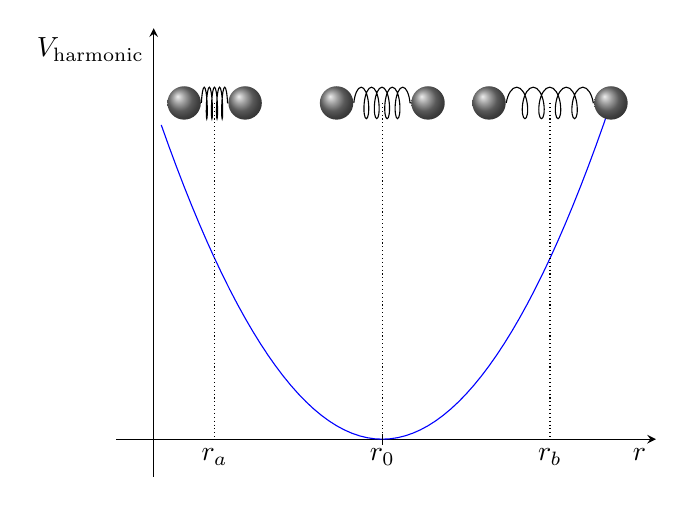
\begin{tikzpicture}
  \begin{axis}[
    grid=none,
    xmax=6,
    ymax=10, 
    axis x line=center,
    axis y line=center,
    restrict y to domain=-1:9,
    enlargelimits,
    xlabel={$r$},
    xlabel style={below left},
    ylabel={$V_{\textrm{harmonic}}$},
    ylabel style={below left},
    ticks=none,
    ]
  \addplot[blue, domain=0.1:10,samples=100] {1*pow(x,2) - 6*x + 9};
  \addplot[mark=|] coordinates {(3,0)} node[below] {$r_0$};

 \draw[densely dotted] (axis cs: 5.2,9 ) --  (axis cs:5.2,0 ) node[below] {$r_b$};
  \draw[densely dotted] (axis cs: 0.8,9 ) --  (axis cs:0.8,0 ) node[below] {$r_a$};
  \draw[densely dotted] (axis cs: 3,9 ) --  (axis cs:3,0 ) node[below] {};

  \addplot[] coordinates {(0.4,9)} node[circle,ball color=gray,inner sep=1.5mm] (a) {};
  \addplot[] coordinates {(1.2,9)} node[circle,ball color=gray,inner sep=1.5mm] (b) {};
  \addplot[] coordinates {(2.4,9)} node[circle,ball color=gray,inner sep=1.5mm] (c) {};
  \addplot[] coordinates {(3.6,9)} node[circle,ball color=gray,inner sep=1.5mm] (d) {};
  \addplot[] coordinates {(4.4,9)} node[circle,ball color=gray,inner sep=1.5mm] (e) {};
  \addplot[] coordinates {(6,9)} node[circle,ball color=gray,inner sep=1.5mm] (f) {};
\draw[draw=black,decoration={aspect=0.1, segment length=0.65mm, amplitude=2mm,coil,},decorate] (a) -- (b); 
\draw[draw=black,decoration={aspect=0.3, segment length=1.32mm, amplitude=2mm,coil,},decorate] (c) -- (d); 
\draw[draw={black},opacity=1,decoration={aspect=0.4, segment length=2.1mm, amplitude=2mm,coil,},decorate] (e) -- (f); 
\end{axis}

\end{tikzpicture}
\end{document}

% Use the following to include the graphics in the chapter
%
%
%\begin{figure}[htbp]
%\begin{center}
%\includegraphics[scale=0.5]{images/fig-ch7_harmonicoscill1.pdf}
%\caption[Caption for list of figures]{Full caption to appear beside the image}
%\label{fig:label}
%\end{center}
%\end{figure}
 